%
% spiegelung.tex -- Kommutator-Regel für D_{\omega t} und S
%
% (c) 2020 Prof Dr Andreas Müller, Hochschule Rapperswil
%
\documentclass[tikz,12pt]{standalone}
\usepackage{times}
\usepackage{amsmath}
\usepackage{txfonts}
\usepackage[utf8]{inputenc}
\usepackage{graphics}
\usepackage{color}
\usepackage{pifont}
\usetikzlibrary{arrows,intersections,math,calc}
\begin{document}

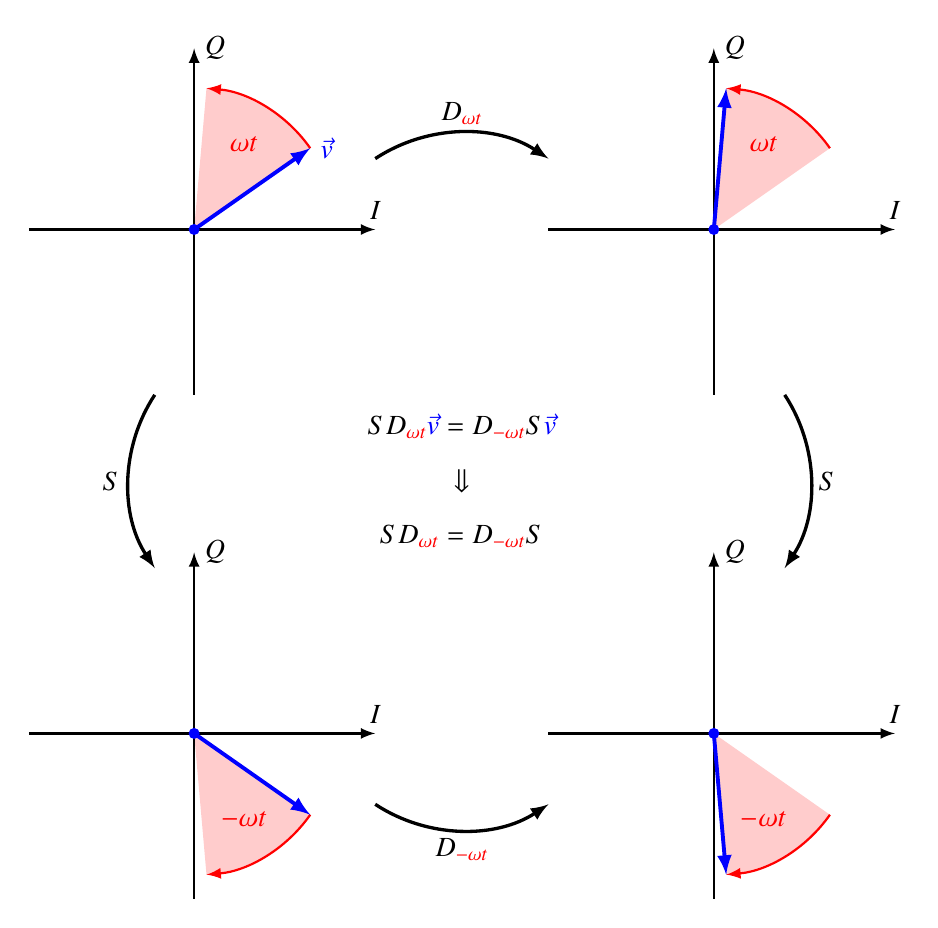
\begin{tikzpicture}[>=latex,thick]

\def\a{35}
\def\b{50}
\def\r{1.8}
\def\s{1.1}
\def\R{2}

\pgfmathparse{asin(\s/\R)}
\xdef\c{\pgfmathresult}

\begin{scope}[xshift=-3.4cm,yshift=3.2cm]
\fill[color=red!20] (0,0) -- ({\r*cos(\a)},{\r*sin(\a)})
	arc ({\a}:{\a+\b}:{\r});
\draw[->] (-2.1,0)--(2.3,0) coordinate[label={$I$}];
\draw[->] (0,-2.1)--(0,2.3) coordinate[label={right:$Q$}];
\draw[->,color=red] ({\r*cos(\a)},{\r*sin(\a)}) arc ({\a}:{\a+\b}:{\r});
\draw[->,color=blue,line width=1.4pt] (0,0)--({\r*cos(\a)},{\r*sin(\a)});
\node[color=blue] at ({\r*cos(\a)},{\r*sin(\a)}) [right] {$\vec{v}$};
\fill[color=blue] (0,0) circle[radius=0.07];
\node[color=red] at ({0.7*\r*cos(\a+0.5*\b))},{0.7*\r*sin(\a+0.5*\b))})
	{$\omega t$};
\end{scope}

\draw[<-,line width=1.2pt] (\s,4.1) arc ({90-\c}:{90+\c}:\R);
\node at (0,4.4) [above] {$D_{\color{red}\omega t}$};

\draw[->,line width=1.2pt] (-\s,-4.1) arc ({-90-\c}:{-90+\c}:\R);
\node at (0,-4.4) [below] {$D_{\color{red}-\omega t}$};

\draw[->,line width=1.2pt] (-3.9,\s) arc ({180-\c}:{180+\c}:\R);
\node at (-4.2,0) [left] {$S$};

\draw[<-,line width=1.2pt] (4.1,-\s) arc ({-\c}:{\c}:\R);
\node at (4.4,0) [right] {$S$};

\begin{scope}[xshift=3.2cm,yshift=3.2cm]
\fill[color=red!20] (0,0) -- ({\r*cos(\a)},{\r*sin(\a)})
	arc ({\a}:{\a+\b}:{\r});
\draw[->] (-2.1,0)--(2.3,0) coordinate[label={$I$}];
\draw[->] (0,-2.1)--(0,2.3) coordinate[label={right:$Q$}];
\draw[->,color=red] ({\r*cos(\a)},{\r*sin(\a)}) arc ({\a}:{\a+\b}:{\r});
\draw[->,color=blue,line width=1.4pt] (0,0)--({\r*cos(\a+\b)},{\r*sin(\a+\b)});
\fill[color=blue] (0,0) circle[radius=0.07];
\node[color=red] at ({0.7*\r*cos(\a+0.5*\b))},{0.7*\r*sin(\a+0.5*\b))})
	{$\omega t$};
\end{scope}

\begin{scope}[xshift=-3.4cm,yshift=-3.2cm]
\fill[color=red!20] (0,0) -- ({\r*cos(\a+\b)},{-\r*sin(\a+\b)})
	arc ({360-\a-\b}:{360-\a}:{\r});
\draw[->] (-2.1,0)--(2.3,0) coordinate[label={$I$}];
\draw[->] (0,-2.1)--(0,2.3) coordinate[label={right:$Q$}];
\draw[<-,color=red] ({\r*cos(\a+\b)},{-\r*sin(\a+\b)})
	arc ({360-\a-\b}:{360-\a}:{\r});
\draw[->,color=blue,line width=1.4pt] (0,0)--({\r*cos(\a)},{-\r*sin(\a)});
\fill[color=blue] (0,0) circle[radius=0.07];
\node[color=red] at ({0.7*\r*cos(\a+0.5*\b))},{-0.7*\r*sin(\a+0.5*\b))})
	{$-\omega t$};
\end{scope}

\begin{scope}[xshift=3.2cm,yshift=-3.2cm]
\fill[color=red!20] (0,0) -- ({\r*cos(\a+\b)},{-\r*sin(\a+\b)})
	arc ({360-\a-\b}:{360-\a}:{\r});
\draw[->] (-2.1,0)--(2.3,0) coordinate[label={$I$}];
\draw[->] (0,-2.1)--(0,2.3) coordinate[label={right:$Q$}];
\draw[<-,color=red] ({\r*cos(\a+\b)},{-\r*sin(\a+\b)})
	arc ({360-\a-\b}:{360-\a}:{\r});
\draw[->,color=blue,line width=1.4pt] (0,0)--({\r*cos(\a+\b)},{-\r*sin(\a+\b)});
\fill[color=blue] (0,0) circle[radius=0.07];
\node[color=red] at ({0.7*\r*cos(\a+0.5*\b))},{-0.7*\r*sin(\a+0.5*\b))})
	{$-\omega t$};
\end{scope}


\node at (0,0.7) {$SD_{\color{red}\omega t}{\color{blue}\vec{v}} = D_{\color{red}-\omega t}S{\color{blue}\vec{v}}$};
\node at (0,0) {$\Downarrow$};
\node at (0,-0.7) {$SD_{\color{red}\omega t} = D_{\color{red}-\omega t}S$};

\end{tikzpicture}

\end{document}

